\section{Results}
\label{sec:results}



% 初期段階の調査として,画像及び動画がissueの各attributesに
% 与える影響について調査する.
% 表2で得られたそれぞれのカテゴリ間で比較を比較を行う.
% 等分散性を仮定できないデータが含まれていたため,
% 比較にはSteel-Dwass testを採用する.
% 
% visualizationは,issueの解決時間,
% コメント数,文字数に何らかの影響を与える.
% 検定結果を表6に示す.
% 有意水準は0.05を採用する.
% IssueResolvedTimeにおいて,
% ImgとMovは片側検定で有意差があった.
% また,表Xより,平均値,中央値でNoneカテゴリの
% issueよりImgとMovカテゴリのissueの方が
% 課題解決時間が長かった.
% よって,画像もしくは動画がissue作成時に付与
% される課題はその解決時間が有意に長くなる.
% また,#comments及び#charsでは両側検定で
% 有意であり,これらのattributesにも
% 有意な影響を与えることがわかった.
% ただし,imageとmovieに有意差は
% 観測されなかった.

% As an initial analysis, we investigated 
% the impact of images and movies on 
% the issues in terms of the attributes. 
% As an initial analysis, 

\subsection{RQ1: \RQone{}}

\begin{figure}[h]
\centering
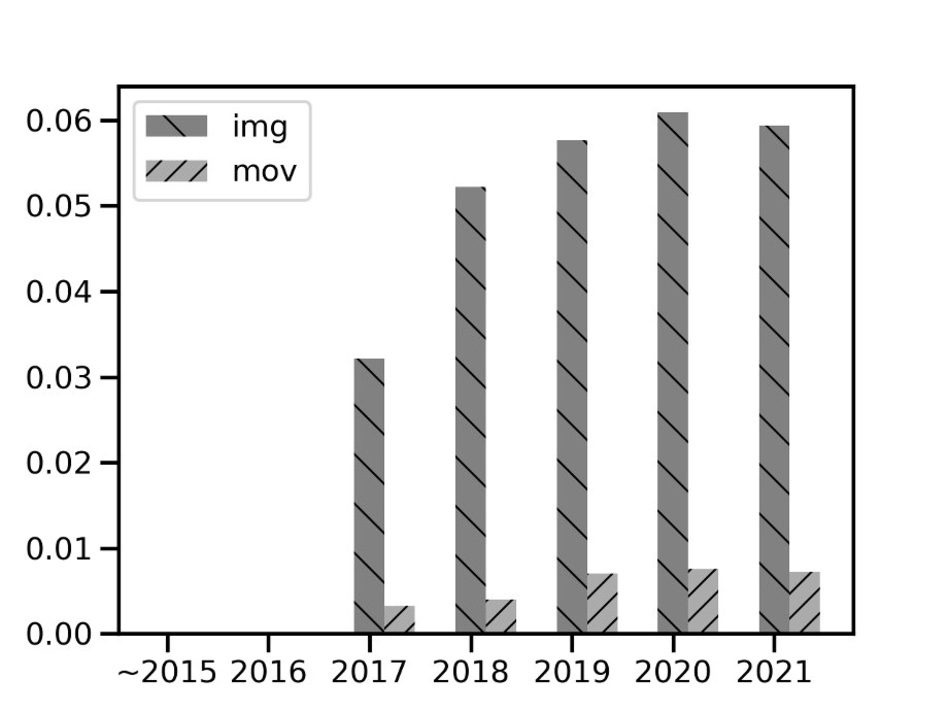
\includegraphics[width=0.6\linewidth]{./figures/data-category-trend.pdf}
\caption{ 
  The proportions of issue reports for each category
  }
\label{fig:data-cat-trend}
\end{figure}

\textbf{Using images and movies is still not popular.}
\fig{fig:data-cat-trend} shows the proportions of 
issues in which developers attach either 
images or movies to the issue descriptions for each year. 
The y-axis shows the proportion. 
We observed that the proportion of the issues 
with movies is less than 1\%. 
Even the proportion of the issues with images is 
around 6\% in 2020 and 2021. 
Hence, the proportion of the issues with either 
images or movies is still low. 
Given this result, both the images and movies are still 
not popular for developers. 

However, the proportions have slightly increased so far 
except for 2021. 
This may be because we collected the resolved issues 
in 2021. 
Hence, using images and movies may be more popular in the future. 


\subsection{RQ2: \RQtwo{}}

\begin{table}[t]
  \begin{center}
  \caption{The Steel-Dwass test results \masa{finally we should remove this table}}
  \begin{tabular}{l r|r}
    \toprule
    Attributes & Category & $p$-value\\
    \midrule
     & \bf{$Img$~vs~$None$} & 0.535 \\
     $IssueResolvedTime$ & \bf{$Mov$~vs~$None$} & 0.636\\
     & \bf{$Img$~vs~$~Mov$} & 0.587 \\
    \midrule
     & \bf{$Img$~vs~$None$} & 0.491 \\
     $FirstCommentTime$ & \bf{$Mov$~vs~$None$} & 0.494 \\
     & \bf{$Img$~vs~$~Mov$} & 0.274 \\
    \midrule
     & \bf{$Img$~vs~$None$} & 0.216 \\
     $\#comments$ & \bf{$Mov$~vs~$None$} & 0.245 \\
     & \bf{$Img$~vs~$~Mov$} & 0.749 \\
    \midrule
     & \bf{$Img$~vs~$None$} & *~~0.002 \\
     $\#words$  & \bf{$Mov$~vs~$None$} &  0.435 \\
     & \bf{$Img$~vs~$~Mov$} & *~~0.012 \\
    \bottomrule
  \end{tabular}\\
  %\small
  % *~ : significant in two-sided test \\
  % ** : significant in one-sided test \\
  \label{tab:Steel-Dwass-test}
  \end{center}
\end{table}
\begin{table*}[t]
  \begin{center}
  \caption{The statistics of the collected issues for each category \masa{finally we should remove this table}}
  % \scalebox{0.85}[0.85]{
  \begin{tabular}{l c c c| c c c| c c c| c c c} 
    \toprule
    & \multicolumn{3}{c}{$ResolutionTime$} & \multicolumn{3}{c}{$FirstCommentTime$} & \multicolumn{3}{c}{$Comments$} & \multicolumn{3}{c}{$DescriptionLengths$}\\
    & \textbf{$Img$} & \textbf{$Vid$} & \textbf{$None$} & \textbf{$Img$} & \textbf{$Vid$} & \textbf{$None$} & \textbf{$Img$} & \textbf{$Vid$} & \textbf{$None$} & \textbf{$Img$} & \textbf{$VId$} & \textbf{$None$} \\ 
    \midrule
    Mean & 32.60 & 40.66   & 40.01   & 8.679 & 14.83 & 13.08 &  3.556 & 3.347 & 3.262 &  104.0 & 104.3 & 149.0 \\
    Min  &       &         &         &       &       &       &        &       &       &        &       &   \\
    25th &       &         &         &       &       &       &        &       &       &        &       &   \\
    50th & 4.784 & 5.698   & 5.946   & 0.239 & 0.395 & 0.318 &  2     & 2     & 2     & 42     & 55    & 60 \\
    75th &       &         &         &       &       &       &        &       &       &  &     & \\
    Max  &       &         &         &       &       &       &        &       &       &  &  &  \\
    S.D. & 63.7  & 76.6    & 72.5    & 32.14 & 48.15 & 41.74 &  4.575 & 4.001 & 5.060 & 431.0 & 202.2 & 592.7 \\
    \bottomrule
  \end{tabular}
  % }
  \label{tab:issue_stat_categories}
  \end{center}
\end{table*}


We investigated 
the differences with and without images and movies 
for each attribute on the issues. 
Specifically, we compared the attributes between 
the categories in \tab{tab:issue-category}. 
Because our preliminary study shows that 
the distributions for each category do not 
come from normal distributions, 
we used a non-parametric test called the \textit{Steel-Dwass test}. 

\textbf{The attribute values are changed 
with and without images and movies.}
\tab{tab:Steel-Dwass-test} shows the results of 
the Steel-Dwass test. 
The asterisks indicate significance based on 
the Steel-Dwass test: * indicates $p$ < 0.05 in 
the two-sided test; 
** indicates $p$ < 0.05 in the one-sided test. 
We observed that the issues in the $Img$ category and 
the $Mov$ category are significantly different from those 
in the $None$ category in terms of $IssueResolvedTime$. 


\tab{tab:issue_stat_categories} shows the statistics
of the collected issues for the $Img$, $Mov$,
and $None$ categories.
The Mean row indicates the average values; 
the Min and Max rows indicate the minimum and maximum values; 
the 25th, 50th, and 75th rows indicate the percentile values; 
the S.D. row indicates the standard deviation values. 
% We may not find the general conclusion; 
% however, we observed differences across the categories. 
% For example, the 25th, 50th, and 75th percentiles of 
% the $Img$ and $Mov$ categories in $IssueResolvedTime$ are 
% longer than those of the $None$ category. 
% % \tab{tab:issue_stat_categories} shows that 
This table shows that 
the mean and the median $IssueResolvedTime$ values of 
the issues in the $Img$ category and the $Mov$ category are 
longer than those in the $None$ category. 
Hence, the issues with images or movies tend to need 
a longer time to be resolved. 

In addition, we observed that the issues in 
the $Img$ category and the $Mov$ category are 
significantly different from those in 
the $None$ category in terms of $\#comments$ and 
$\#chars$. 
Hence, the issues with images or movies 
tend to have different numbers of 
comments and words in the issue description.

It should be noted that we do not observe 
the difference between the $Img$ category and 
the $Mov$ category. 



\begin{table}[t]
  \begin{center}
  % \caption{The top-10 words in terms of TFIDF}
  \caption{Top-10 words in terms of TFIDF}
  \begin{tabular}{r | c c c}
    \hline
     & $Img$ & $Vid$ & $None$\\
    \hline
    1 & image & packages & file\\
    2 & error & view & error\\
    3 & screenshot & when & lib\\
    4 & when & python & if\\
    5 & have & pageviewcontroller & line\\
    6 & if & config & java \\
    7 & version & local & get\\
    8 & get & version & have\\
    9 & using & problem & when\\
    10& file & error & version\\
    \hline
  \end{tabular}\\
  \label{tab:tfidf-result}
  \end{center}
\end{table}


% We used $Words$ to compute the TFIDF values\masa{need citation} for each category. 
% The TFIDF values will support researchers who investigate 
% the differences in the appearances of words with and without 
% images/movies. 
We suppose that images and movies are utilized to 
describe specific contents such as GUI bugs. 
Hence, we computed the TFIDF values\masa{need citation} 
on $Words$ for each category. 
The TFIDF values clarify the differences in the appearances of 
words with and without images/movies. 

\textbf{The issues with either images or movies have 
more words about visualization or GUI.}
\tab{tab:tfidf-result} shows the top-10 TFIDF words
% in $Words$ 
for each category.
It should be noted that we remove a kind of stop words such as 
``at'', ``it'', and ``the''. 
% extracted from our dataset. 
We observed words related to visualization such as 
``image'' and ``view'' in the $Img$ and $Mov$ categories. 
Also, we observed words related to GUI such as 
``dropdown'' and ``button'' in the $Mov$ category. 
The word ``when'' indicates high TFIDF values 
in the $Img$ and $Mov$ categories. 
Our manual analysis reveals that the issues with 
these words relate to reporting bugs. 
Hence, the issues in these two categories are 
probably more related to reporting bugs. 
